\section{Generación de señalamiento paso a paso}

	Inicialmente, el RNA ejecuta el Algoritmo \ref{alg:graph_network} (ver Sección \ref{sec:grafos}) para detectar todos los \textit{netElements}, sus coordenadas iniciales y finales en la topología, y el sentido en el que fueron definidas. Al concluir el Algoritmo \ref{alg:graph_network}, el RNA ejecuta el Algoritmo \ref{alg:connectedness} (ver Sección \ref{sec:grafos}) para analizar la conexidad de la red. El resultado obtenido se muestra en el Código \ref{lst:EJ5_1}, donde se describen las coordenadas de cada \textit{netElement} y se confirma que la red es conexa.
	
	\begin{lstlisting}[language = {}, caption = Detección de \textit{netElements} por parte del RNA , label = {lst:EJ5_1}]
		###### Starting Railway Network Analyzer #####
		Reading .railML file
		Creating railML object
		Analyzing railML object
		Analyzing graph
		ne01 [-1451, -150] [-763, -150] >>
		ne02 [-763, -150] [736, -150] >>
		ne03 [-763, -150] [736, -150] >>
		ne04 [736, -150] [1451, -150] >>
		ne05 [-1451, -450] [-763, -450] >>
		ne06 [-763, -450] [736, -450] >>
		ne07 [-763, -450] [736, -450] >>
		ne08 [736, -450] [1451, -450] >>
		The network is not connected
	\end{lstlisting}
	
	Por ejemplo, el \textit{netElement} ne08 inicia en la coordenada (736;-450) y finaliza en la coordenada (1451;-450). El símbolo $>>$ indica que ne08 se encuentra definido de izquierda a derecha, ya que la componente x de la coordenada final es mayor a la de la coordenada inicial, teniendo la misma componente y. Además, se puede comprobar que la lista obtenida en consistente con la Figura \ref{fig:EJ5_2}. Por ejemplo, ne01, ne02 y ne03 comparten la coordenada (736;-450), que coincide con la coordenada del cambio de vías Sw01.
	
	A continuación, el RNA detectará la infraestructura ferroviaria, las curvas peligrosas y los puntos medios de los netElements que el RNA considera demasiado largos. El análisis de la infraestructura se detalla en la Sección \ref{sec:bufferstop}, Sección \ref{sec:detectors}, Sección \ref{sec:platform} y Sección \ref{sec:crossing}, mientras que la detección de curvas y puntos medios se detalla en la Sección \ref{sec:tracks}. El RNA ejecuta el Algoritmo \ref{alg:switches_1}, Algoritmo \ref{alg:switches_2} y Algoritmo \ref{alg:switches_3} para confirmar la detección de cambios de vías simples, dobles y en tijeras. El resultado de este proceso se puede visualizar en el Código \ref{lst:EJ5_2}.
	
	\begin{lstlisting}[language = {}, caption = Detección de puntos críticos por parte del RNA , label = {lst:EJ5_2}]
	Analyzing infrastructure --> Infrastructure.RNA
	Detecting Danger --> Safe_points.RNA
	ne01 has a RailJoint[J01] @ [-1101, -150]     
	ne02 has a Middle point @ [-548.9, -150]      
	ne02 has a Middle point @ [-334.7, -150]      
	ne02 has a Middle point @ [-120.6, -150]
	ne02 has a Middle point @ [93.6, -150]
	ne02 has a Middle point @ [307.7, -150]
	ne02 has a Middle point @ [521.9, -150]
	ne03 has a RailJoint[J05] @ [-11, 150]
	ne03 has a Curve(3 lines) @ [[-463, 150], [436, 150]]
	ne04 has a RailJoint[J08] @ [1100, -150]
	ne05 has a RailJoint[J09] @ [-1118, -450]
	ne06 has a Middle point @ [-548.9, -450]
	ne06 has a Middle point @ [-334.7, -450]
	ne06 has a Middle point @ [-120.6, -450]
	ne06 has a Middle point @ [93.6, -450]
	ne06 has a Middle point @ [307.7, -450]
	ne06 has a Middle point @ [521.9, -450]
	ne07 has a RailJoint[J12] @ [-5, -750]
	ne07 has a Curve(3 lines) @ [[-463, -750], [436, -750]]
	ne08 has a RailJoint[J16] @ [1100, -450]
	\end{lstlisting}
	
	Esta información es exportada por el RNA, con mayor detalle, en el archivo Infrastructure.RNA (Código \ref{lst:EJ5_4}) que resume cada elemento ferroviario asociado a su respectivo \textit{netElement}.
	
	\begin{lstlisting}[language = {}, caption = Infrastructure.RNA, label = {lst:EJ5_4}]
Nodes: 8|Switches: 4|Signals: 0|Detectors: 6|Ends: 4|Barriers: 0
Node ne01:
	Track = track1
	TrainDetectionElements -> tde89
		Type -> insulatedRailJoint
		Type = BufferStop -> ['bus174']
	Neighbours = 2 -> ['ne02', 'ne03']
	Switches -> Sw01
		ContinueCourse -> right -> ne02
		BranchCourse -> left -> ne03
Node ne02:
	Track = track5
	Neighbours = 3 -> ['ne01', 'ne03', 'ne04']
Node ne03:
	Track = track6
		TrainDetectionElements -> tde93
		Type -> insulatedRailJoint
	Neighbours = 3 -> ['ne01', 'ne02', 'ne04']
Node ne04:
	Track = track3
	TrainDetectionElements -> tde96
		Type -> insulatedRailJoint
		Type = BufferStop -> ['bus176']
	Neighbours = 2 -> ['ne02', 'ne03']
	Switches -> Sw02
		ContinueCourse -> left -> ne02
		BranchCourse -> right -> ne03
Node ne05:
	Track = track2
	TrainDetectionElements -> tde105
		Type -> insulatedRailJoint
		Type = BufferStop -> ['bus175']
	Neighbours = 2 -> ['ne06', 'ne07']
	Switches -> Sw03
		ContinueCourse -> left -> ne06
		BranchCourse -> right -> ne07
Node ne06:
	Track = track7
	Neighbours = 3 -> ['ne05', 'ne07', 'ne08']
Node ne07:
	Track = track8
	TrainDetectionElements -> tde108
		Type -> insulatedRailJoint
	Neighbours = 3 -> ['ne05', 'ne06', 'ne08']
Node ne08:
	Track = track4
	TrainDetectionElements -> tde112
		Type -> insulatedRailJoint
		Type = BufferStop -> ['bus177']
	Neighbours = 2 -> ['ne06', 'ne07']
	Switches -> Sw04
		ContinueCourse -> right -> ne06
		BranchCourse -> left -> ne07
	\end{lstlisting}	
	
	La información de la infraestructura es utilizada por el RNA para detectar los puntos críticos de la red, es decir, las zonas donde es recomendable colocar una señal, según el sentido de circulación que se desee. El resultado es exportado al archivo SafePoints.RNA (Código \ref{lst:EJ5_5}). En el caso de que un mismo \textit{netElement} tenga más de un punto crítico para el mismo sentido, el RNA tomará el más cercano al elemento a proteger. El criterio de selección de puntos críticos se aplica para cada elemento ferroviario detectado, cada curva y cada cambio de vías y fue explicado en las secciones correspondientes ya mencionadas.
	
	\begin{lstlisting}[language = {}, caption = SafePoints.RNA, label = {lst:EJ5_5}]
ne01:
	Next: [[-1201.0, -150]]
	Prev: [[-1001.0, -150]]
ne02:
	Next: [[-548.9, -150], [-334.7, -150], [-120.6, -150], [93.6, -150], [307.7, -150], [521.9, -150]]
	Prev: [[-548.9, -150], [-334.7, -150], [-120.6, -150], [93.6, -150], [307.7, -150], [521.9, -150]]
ne03:
	Next: [[-111.0, 150], [336.0, 150]]
	Prev: [[89.0, 150], [-363.0, 150]]
ne04:
	Next: [[1000.0, -150]]
	Prev: [[1200.0, -150]]
ne05:
	Next: [[-1218.0, -450]]
	Prev: [[-1018.0, -450]]
ne06:
	Next: [[-548.9, -450], [-334.7, -450], [-120.6, -450], [93.6, -450], [307.7, -450], [521.9, -450]]
	Prev: [[-548.9, -450], [-334.7, -450], [-120.6, -450], [93.6, -450], [307.7, -450], [521.9, -450]]
ne07:
	Next: [[-105.0, -750], [336.0, -750]]
	Prev: [[95.0, -750], [-363.0, -750]]
ne08:
	Next: [[1000.0, -450]]
	Prev: [[1200.0, -450]]
	\end{lstlisting}	
	
	Una vez que el RNA detectó cada punto crítico de la red ferroviaria, procede a generar el señalamiento. El orden en que se procesan los elementos ferroviarios no impacta en el resultado final, pero para poder describirlo de forma ordenada se iniciará generando el señalamiento para proteger los finales de vías, las junturas entre rieles, las plataformas (explicado en la Sección \ref{sec:sig_platform}), los cruces de vía (explicado en la Sección \ref{sec:sig_levelcrossing}) y los cambios de vías (explicado en la Sección \ref{sec:signal_switches}). Luego se procederá a mostrar el señalamiento completo antes y después de la simplificación de señales (explicado en la Sección \label{sec:simplificacion}). 
	
	Tal cómo se explicó en la Sección \ref{sec:sig_border}, el RNA aplica el Algoritmo \ref{alg:lineBorder} y el Algoritmo \ref{alg:bufferStop} para generar las señales para proteger los finales de vías relativos y absolutos. Estas señales son ilustradas en la Figura \ref{fig:EJ5_3}.

	\begin{figure}[H]
		\centering
		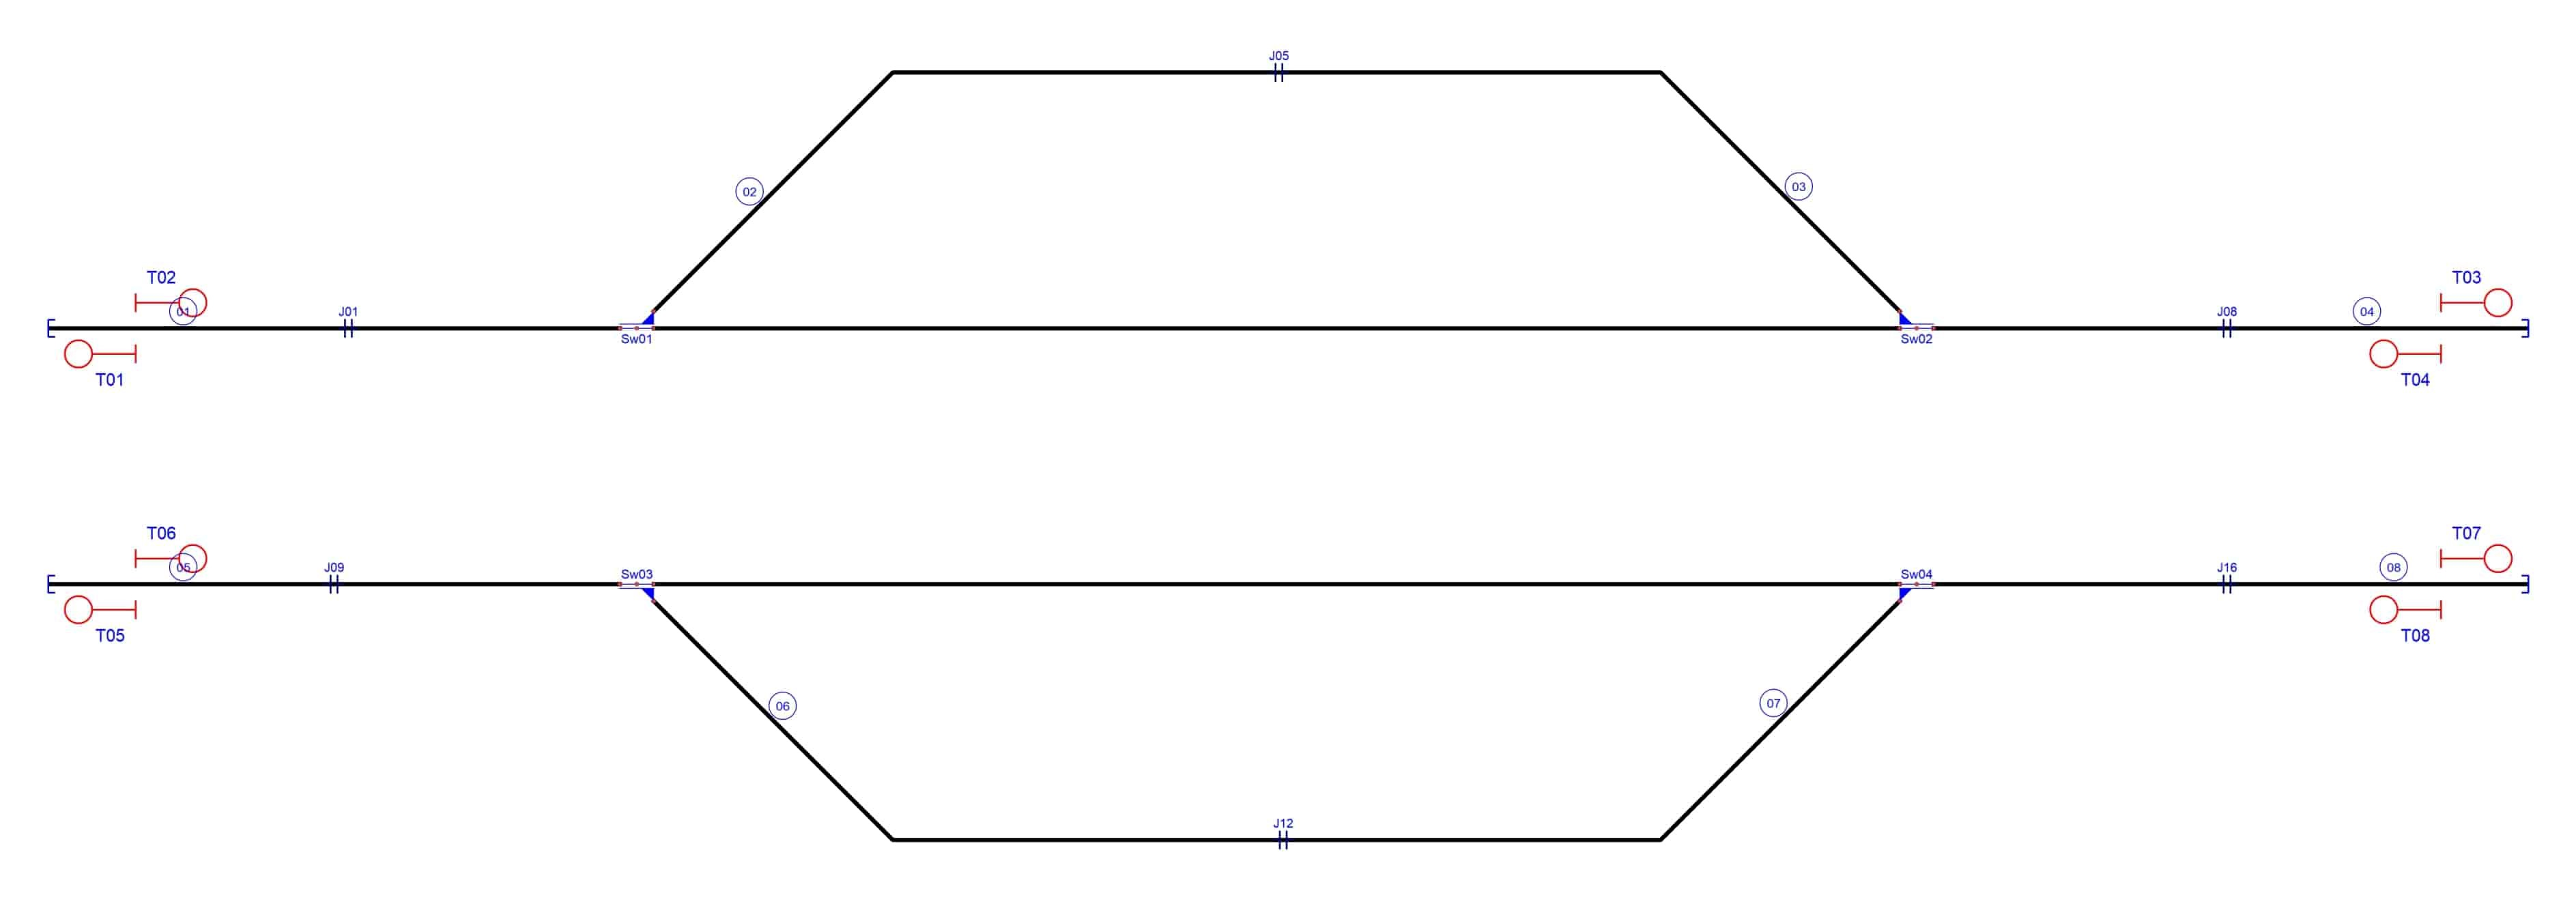
\includegraphics[width=1\textwidth]{resultados-obtenidos/ejemplo5/images/5_step1.png}
		\centering\caption{Señalamiento generado por el RNA para proteger el fin de vía.}
		\label{fig:EJ5_3}
	\end{figure}
	
	Los finales de vías absolutos son protegidos por las señales de parada T01, T03, T05 y T07, y las señales de partida son T02, T04, T06 y T08. No existen finales de vías relativos que proteger.
	
	La Figura \ref{fig:EJ5_4} ilustra la generación de señales destinadas a proteger las junturas entre los rieles. Estas señales se obtuvieron al aplicar el Algoritmo \ref{alg:RJ}, tal como fue explicado en la Sección \ref{sec:sig_joint}. Las señales generadas son todas las señales entre J09 y J20, indicadas en color rojo.	
	
	\begin{figure}[H]
		\centering
		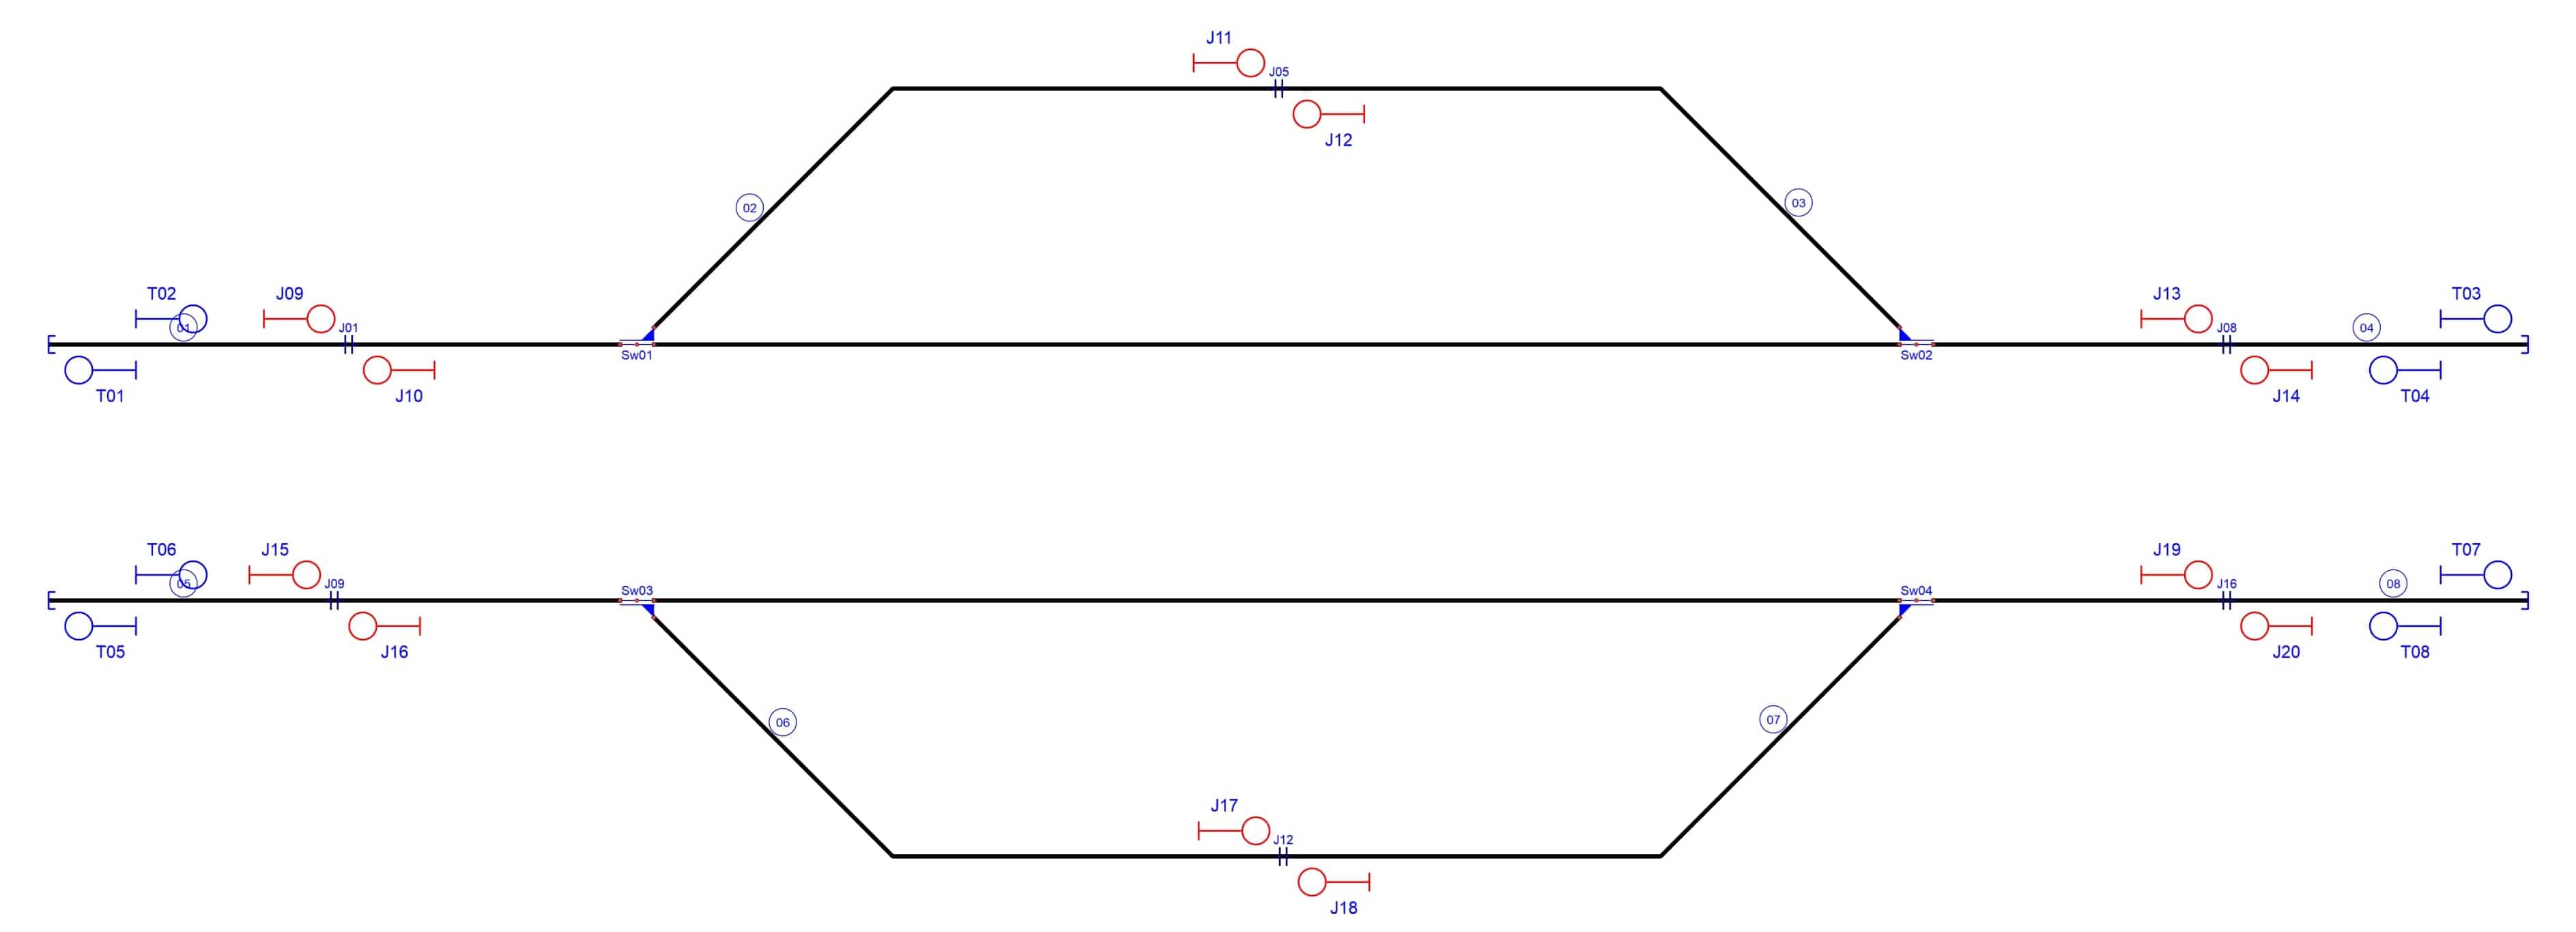
\includegraphics[width=1\textwidth]{resultados-obtenidos/ejemplo5/images/5_step2.png}
		\centering\caption{Señalamiento generado por el RNA para proteger las junturas.}
		\label{fig:EJ5_4}
	\end{figure}
	
	Al generar el señalamiento para proteger la infraestructura, tal como se explicó en la Sección \ref{sec:horizontal}, el Algoritmo \ref{alg:horizontal} simplificará las señales entre dos elementos ferroviarios si no existe espacio suficiente entre ellos. El señalamiento generado para proteger las plataformas y los cruces de vía, producto de aplicar el Algoritmo \ref{alg:PTF} y el Algoritmo \ref{alg:LC}, respectivamente, se ilustra en roj en la Figura \ref{fig:EJ5_5}. Al no existir plataformas o cruces de vías que proteger, ninguna señal fue generada por el RNA.
	
	\begin{figure}[H]
		\centering
		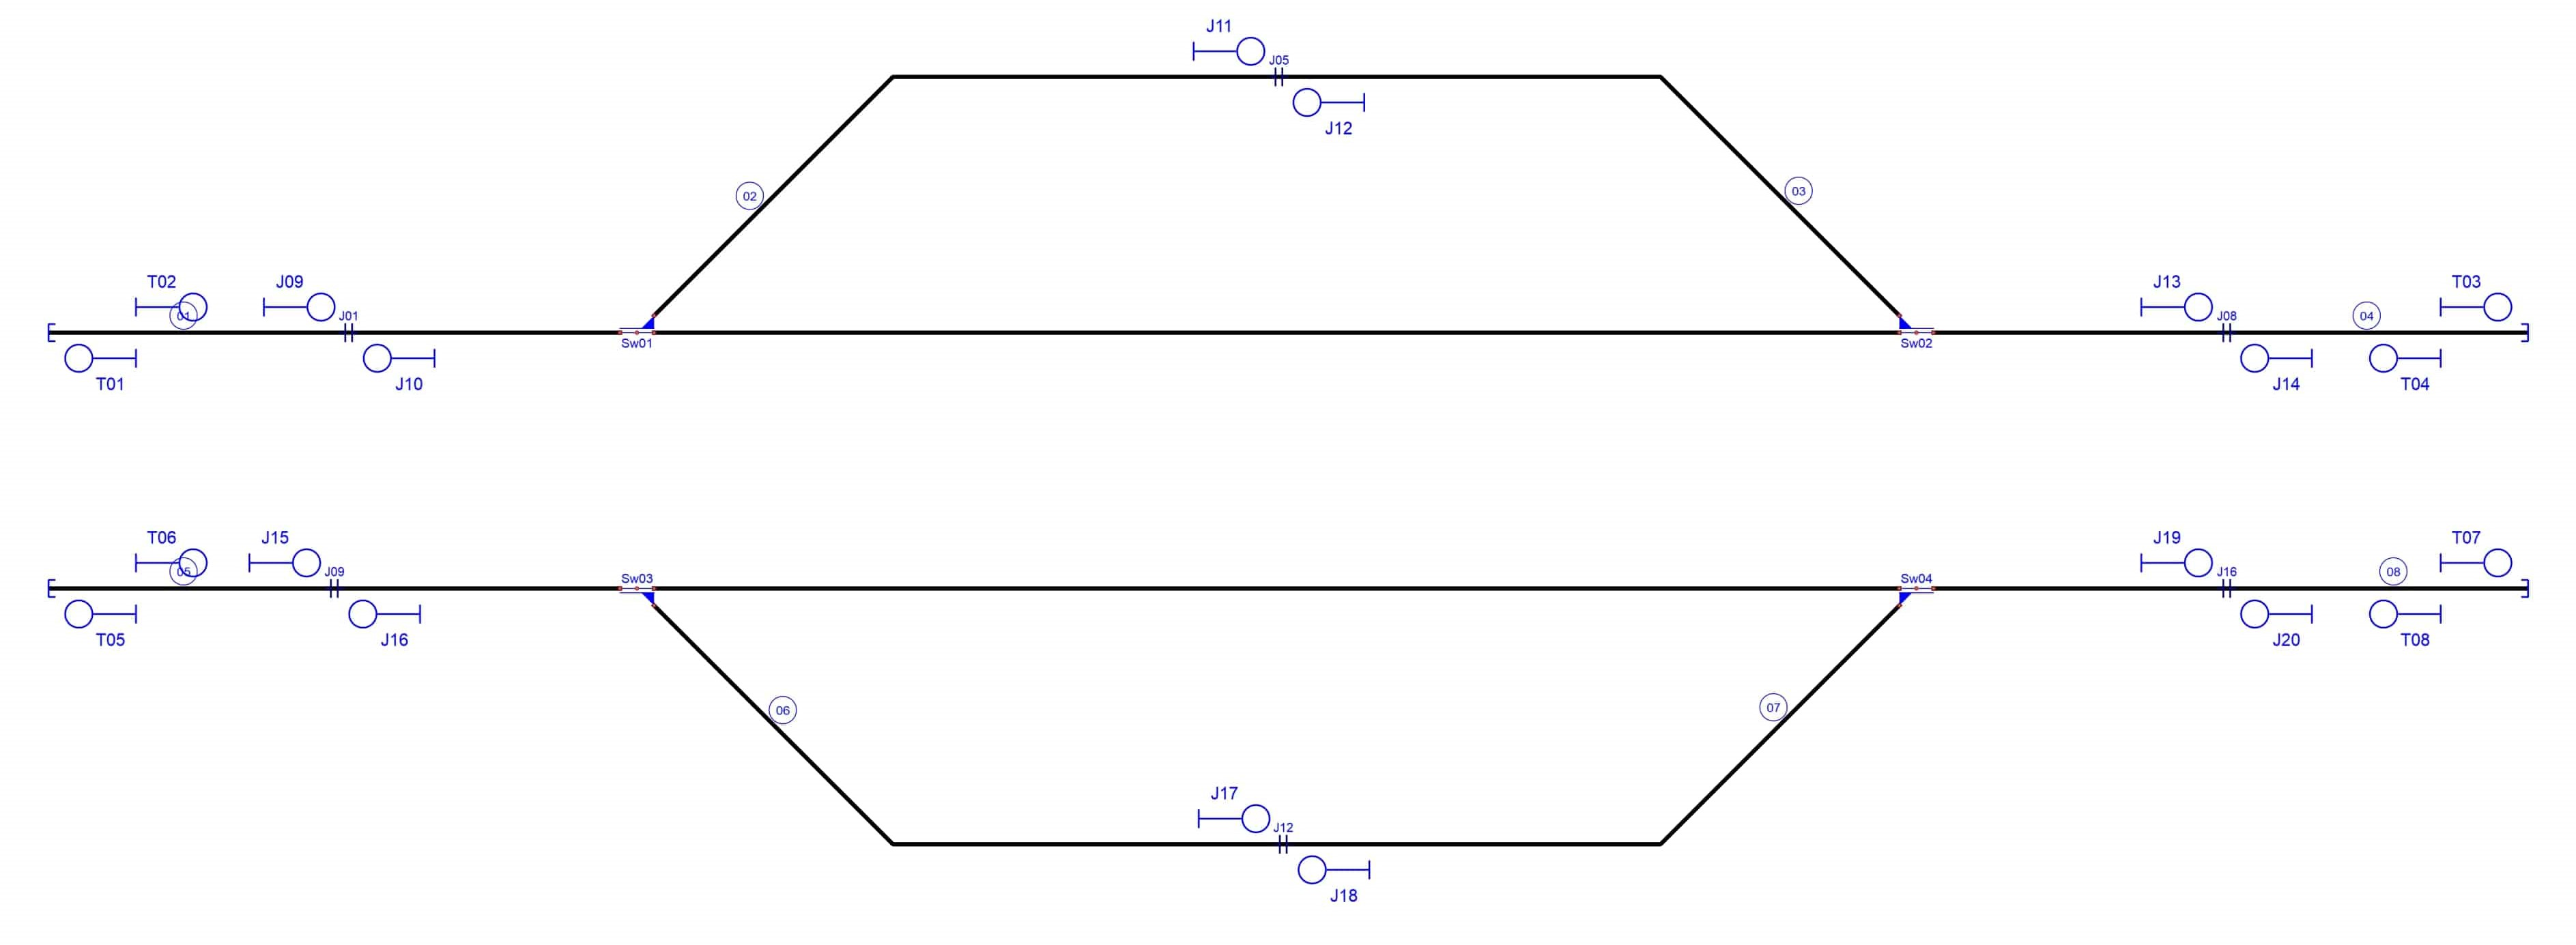
\includegraphics[width=1\textwidth]{resultados-obtenidos/ejemplo5/images/5_step3.png}
		\centering\caption{Señalamiento generado por el RNA para proteger plataformas y cruces de vía.}
		\label{fig:EJ5_5}
	\end{figure}
	
	Al aplicar el Algoritmo \ref{alg:SW} de generación de señalamiento para cambios de vías, tal como fue explicado en la Sección \label{sec:signal_switches}, el RNA genera las señales C21, S23, B26 y H24 para proteger el cambio de vías Sw02; las señales C25, S27, B22 y H28 para proteger el cambio de vías Sw02; las señales C29, S31. B34 y H32 para proteger el cambio de vías Sw03 y las señales C33, S35, B30 y H36 para proteger el cambio de vías Sw04. Las señales mencionadas se encuentran resaltadas en rojo en la Figura \ref{fig:EJ5_6}.
	
	\begin{figure}[H]
		\centering
		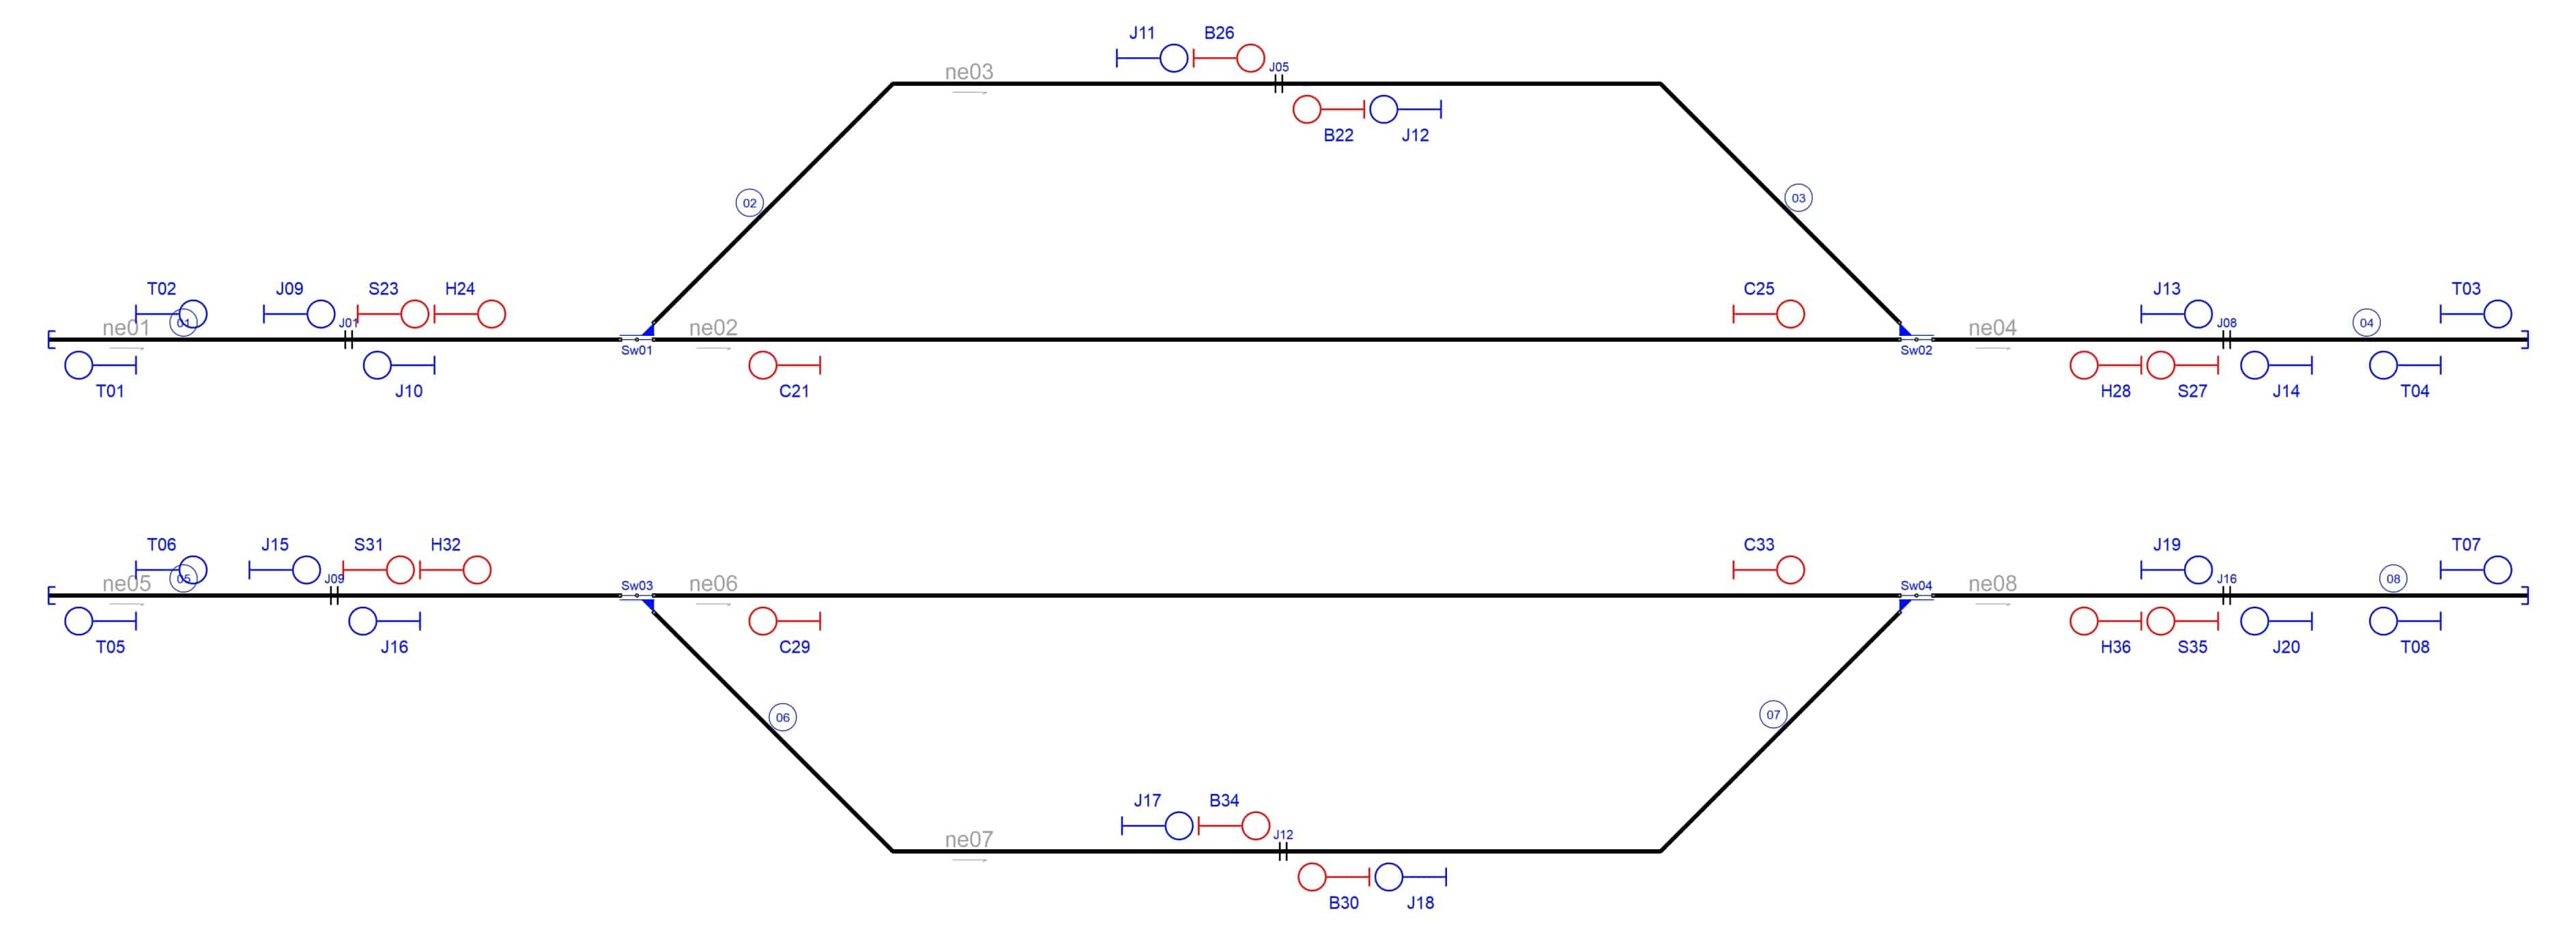
\includegraphics[width=1\textwidth]{resultados-obtenidos/ejemplo5/images/5_step4.png}
		\centering\caption{Señalamiento generado por el RNA para proteger los cambios de vías.}
		\label{fig:EJ5_6}
	\end{figure}
	
	Una vez obtenido todo el señalamiento, el RNA procede a simplificar las señales redundantes, repetidas o cuyas funciones o ubicaciones se superponen entre sí. El proceso de simplificación de señales fue explicado en la Sección \ref{sec:simplificacion}. En este ejemplo, el Algoritmo \ref{alg:vertical} de herencia vertical no fue aplicado, al no cumplirse las condiciones de aplicación.
	
	Las señales simplificadas al aplicar el Algoritmo \ref{alg:horizontal} de herencia horizontal son: J09, J10, J11, J12, J13, J14, J15, J16, J17, J18, S23, H24, S27, H28, S31, H32, S35 y H23. Las señales J09, S23 y H24 fueron eliminadas por su cercanía con la señal T02, con la cual comparten dirección y sentido. Lo mismo ocurre entre las señales J14, S27 y H28, borradas por la señal T04; entre las señales J15, S31 y H32, borradas por la señal T06; entre las señales J20, S35 y H36, borradas por la señal T08;entre la señal J10 y la señal T01; la señal J13 y la señal T03; la señal J16 y la señal T05; y entre la señal J19 y la señal T07. En todos los casos, se aplicó el Algoritmo \ref{alg:horizontal}, diseñado para agrupar objetos cercanos como un único objeto, generando el señalamiento acorde a los elementos contenidos en cada extremo del nuevo elemento contenedor.
	
	Finalmente, las señales son simplificadas aplicando el Algoritmo \ref{alg:reduction} de eliminación por prioridad de señales. El resultado de este proceso es detallado en el Código \ref{lst:EJ5_3}.
	
	\begin{lstlisting}[language = {}, caption = Reducción de señalamiento por prioridad de señales, label = {lst:EJ5_3}]
	Reducing redundant signals
	removing sig10 for sig01
	removing sig09 for sig02
	removing sig23 for sig02
	removing sig24 for sig02
	removing sig13 for sig03
	removing sig14 for sig04
	removing sig27 for sig04
	removing sig28 for sig04
	removing sig16 for sig05
	removing sig15 for sig06
	removing sig31 for sig06
	removing sig32 for sig06
	removing sig19 for sig07
	removing sig20 for sig08
	removing sig35 for sig08
	removing sig36 for sig08
	removing sig11 for sig26
	removing sig12 for sig22
	removing sig17 for sig34
	removing sig18 for sig30
	\end{lstlisting}
	
	El resultado de la simplificación del señalamiento se ilustra en la Figura \ref{fig:EJ5_7}.
	
	\begin{figure}[H]
		\centering
		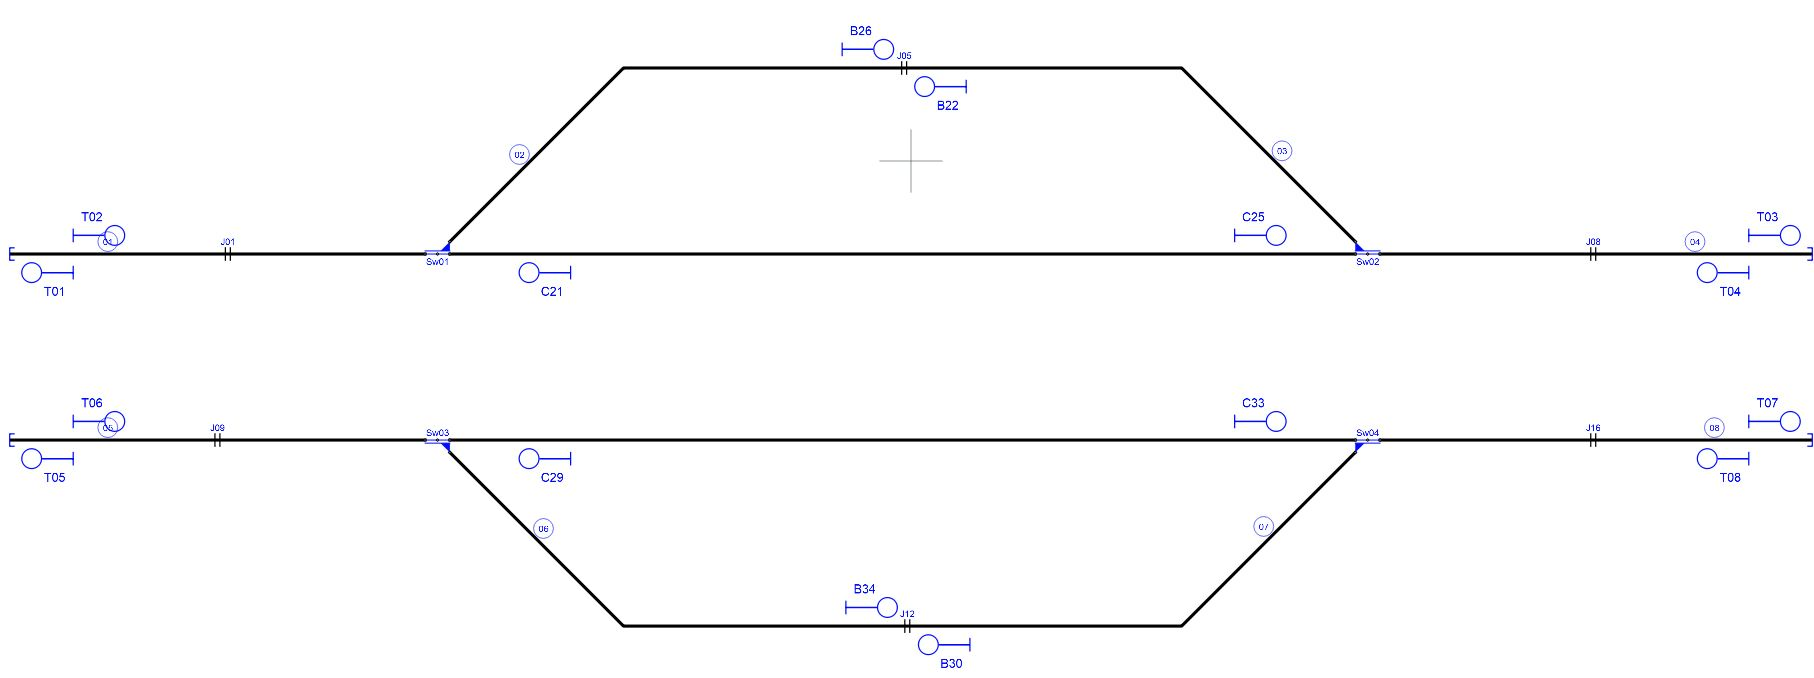
\includegraphics[width=1\textwidth]{resultados-obtenidos/ejemplo5/images/5_RNA.png}
		\centering\caption{Señalamiento generado y simplificado por el RNA.}
		\label{fig:EJ5_7}
	\end{figure}
	
	Además, toda la información del señalamiento generado es exportada por el RNA en el archivo Signalling.RNA (Código \ref{lst:EJ5_6}), que incluye información detallada de la posición, orientación, sentido, coordenada, nombre y tipo de señal.
	
	\begin{lstlisting}[language = {}, caption = Signalling.RNA, label = {lst:EJ5_6}]
sig01 [T01] <<:
	From: ne01 | To: bus174_left
	Type: Stop | Direction: reverse | AtTrack: right 
	Position: [-1351, 150] | Coordinate: 0.1453
sig02 [T02] >>:
	From: ne01 | To: ne01_right
	Type: Stop | Direction: normal | AtTrack: left 
	Position: [-1351, 150] | Coordinate: 0.1453
sig03 [T03] >>:
	From: ne04 | To: bus176_right
	Type: Stop | Direction: normal | AtTrack: left 
	Position: [1351, 150] | Coordinate: 0.8601
sig04 [T04] <<:
	From: ne04 | To: ne04_left
	Type: Stop | Direction: reverse | AtTrack: right 
	Position: [1351, 150] | Coordinate: 0.8601
sig05 [T05] <<:
	From: ne05 | To: bus175_left
	Type: Stop | Direction: reverse | AtTrack: right 
	Position: [-1351, 450] | Coordinate: 0.1453
sig06 [T06] >>:
	From: ne05 | To: ne05_right
	Type: Stop | Direction: normal | AtTrack: left 
	Position: [-1351, 450] | Coordinate: 0.1453
sig07 [T07] >>:
	From: ne08 | To: bus177_right
	Type: Stop | Direction: normal | AtTrack: left 
	Position: [1351, 450] | Coordinate: 0.8601
sig08 [T08] <<:
	From: ne08 | To: ne08_left
	Type: Stop | Direction: reverse | AtTrack: right 
	Position: [1351, 450] | Coordinate: 0.8601
sig21 [C21] <<:
	From: ne02 | To: ne02_left
	Type: Circulation | Direction: reverse | AtTrack: right 
	Position: [-548.9, 150] | Coordinate: 0.1428
sig22 [B22] <<:
	From: ne03 | To: ne03_left
	Type: Manouver | Direction: reverse | AtTrack: right 
	Position: [89.0, -150] | Coordinate: 0.8014
sig25 [C25] >>:
	From: ne02 | To: ne02_right
	Type: Circulation | Direction: normal | AtTrack: left 
	Position: [521.9, 150] | Coordinate: 0.8571
sig26 [B26] >>:
	From: ne03 | To: ne03_right
	Type: Manouver | Direction: normal | AtTrack: left 
	Position: [-111.0, -150] | Coordinate: 0.6869
sig29 [C29] <<:
	From: ne06 | To: ne06_left
	Type: Circulation | Direction: reverse | AtTrack: right 
	Position: [-548.9, 450] | Coordinate: 0.1428
sig30 [B30] <<:
	From: ne07 | To: ne07_left
	Type: Manouver | Direction: reverse | AtTrack: right 
	Position: [95.0, 750] | Coordinate: 0.8048
sig33 [C33] >>:
	From: ne06 | To: ne06_right
	Type: Circulation | Direction: normal | AtTrack: left 
	Position: [521.9, 450] | Coordinate: 0.8571
sig34 [B34] >>:
	From: ne07 | To: ne07_right
	Type: Manouver | Direction: normal | AtTrack: left 
	Position: [-105.0, 750] | Coordinate: 0.6904
	\end{lstlisting}	
	
	Al finalizar la generación del señalamiento, el RNA ejecuta el Algoritmo \ref{alg:routes}, explicado en la Sección \ref{sec:rutas}, para detectar todas las posibles rutas admitidas por la red para crear la tabla de enclavamientos. La cuál puede ser visualizada en el archivo Routes.RNA (Código \ref{lst:EJ5_7}). La misma detalla las señales de inicio y final, los \textit{netElements} abarcados por la ruta y cualquier infraestructura involucrada, incluyendo el estado que deben tener para que la ruta sea activada.
	
	\begin{lstlisting}[language = {}, caption = Routes.RNA, label = {lst:EJ5_7}]
route_1 [sig02 >> sig25]:
	Path: ['ne01', 'ne02']
	Switches: ['Sw01']
route_2 [sig02 >> sig26]:
	Path: ['ne01', 'ne03']
	Switches: ['Sw01']
route_3 [sig04 << sig21]:
	Path: ['ne04', 'ne02']
	Switches: ['Sw02']
route_4 [sig04 << sig22]:
	Path: ['ne04', 'ne03']
	Switches: ['Sw02']
route_5 [sig06 >> sig33]:
	Path: ['ne05', 'ne06']
	Switches: ['Sw03']
route_6 [sig06 >> sig34]:
	Path: ['ne05', 'ne07']
	Switches: ['Sw03']
route_7 [sig08 << sig29]:
	Path: ['ne08', 'ne06']
	Switches: ['Sw04']
route_8 [sig08 << sig30]:
	Path: ['ne08', 'ne07']
	Switches: ['Sw04']
route_9 [sig21 << sig01]:
	Path: ['ne02', 'ne01']
	Switches: ['Sw01']
route_10 [sig22 << sig01]:
	Path: ['ne03', 'ne01']
	Switches: ['Sw01']
route_11 [sig25 >> sig03]:
	Path: ['ne02', 'ne04']
	Switches: ['Sw02']
route_12 [sig26 >> sig03]:
	Path: ['ne03', 'ne04']
	Switches: ['Sw02']
route_13 [sig29 << sig05]:
	Path: ['ne06', 'ne05']
	Switches: ['Sw03']
route_14 [sig30 << sig05]:
	Path: ['ne07', 'ne05']
	Switches: ['Sw03']
route_15 [sig33 >> sig07]:
	Path: ['ne06', 'ne08']
	Switches: ['Sw04']
route_16 [sig34 >> sig07]:
	Path: ['ne07', 'ne08']
	Switches: ['Sw04']
	\end{lstlisting}
	
	
	
	